\section{Experiments and Comprehensive Analysis}

To empirically validate the superiority of XHBot against relation camouflage, we conducted a rigorous suite of experiments across three distinct, large-scale bot detection benchmarks.

\subsection{Experimental Setup}

\subsubsection{Evaluation Datasets}
We evaluate our framework on three widely adopted benchmarks that represent distinct eras and scales of bot evolution:
\begin{itemize}
    \item \textbf{TwiBot-20}~\cite{feng2021twibot20}: A comprehensive graph-based benchmark containing 229,573 users and 455,958 follow relationships. With a bot ratio of roughly 29\%, it serves as the primary standard for modern relational GNN comparison.
    \item \textbf{TwiBot-22}~\cite{feng2022twibot22}: The largest heterogeneous information network benchmark available, scaling to $\sim$1,000,000 users and over 170 million relationships across four node types and six edge types. This dataset explicitly tests the scalability and multi-relational capacity of XHBot.
    \item \textbf{Cresci-2017}~\cite{cresci2017paradigm}: A legacy dataset featuring distinct families of social spambots (e.g., traditional vs. third-generation). It provides a high-density, high-imbalance environment ($\sim$68\% bots) to validate heterophily resilience against specific, known bot-ring topologies.
\end{itemize}

\subsubsection{Evaluation Metrics}
We utilize a robust suite of metrics to evaluate both detection performance and forensic transparency.
\begin{itemize}
    \item \textbf{Bot Detection Performance:} We report F1 Score, Area Under the Receiver Operating Characteristic Curve (AUC-ROC), Accuracy, and the Matthews Correlation Coefficient (MCC). Following established protocols, \textbf{F1 Score} serves as our primary comparative metric due to severe class imbalance.
    \item \textbf{Explanation Quality Metrics:} To validate the Hierarchical Forensic Explanation (HFE) module, we evaluate \textbf{Fidelity+} (accuracy drop when the explanation subgraph is removed), \textbf{Fidelity-} (accuracy when only the subgraph is retained), and \textbf{Sparsity} (conciseness of the explanation).
\end{itemize}

\subsubsection{Hyperparameter Settings and Computational Efficiency}
Models were implemented using PyTorch Geometric and trained on an NVIDIA A100 GPU. The hidden channel dimension was set to $d_h = 64$. We optimized using Adam (learning rate 0.01, weight decay $10^{-4}$) for 200 epochs. Regarding computational efficiency, XHBot maintains a highly competitive footprint: training requires only 4.2 seconds per epoch on TwiBot-20, with inference completing in sub-millisecond latencies per node, ensuring feasibility for real-world deployment.

\subsection{Quantitative Performance Comparison}
The primary classification performance across all three benchmark datasets is detailed in Figure \ref{fig:comparison}.

\begin{figure}[h]
    \centering
    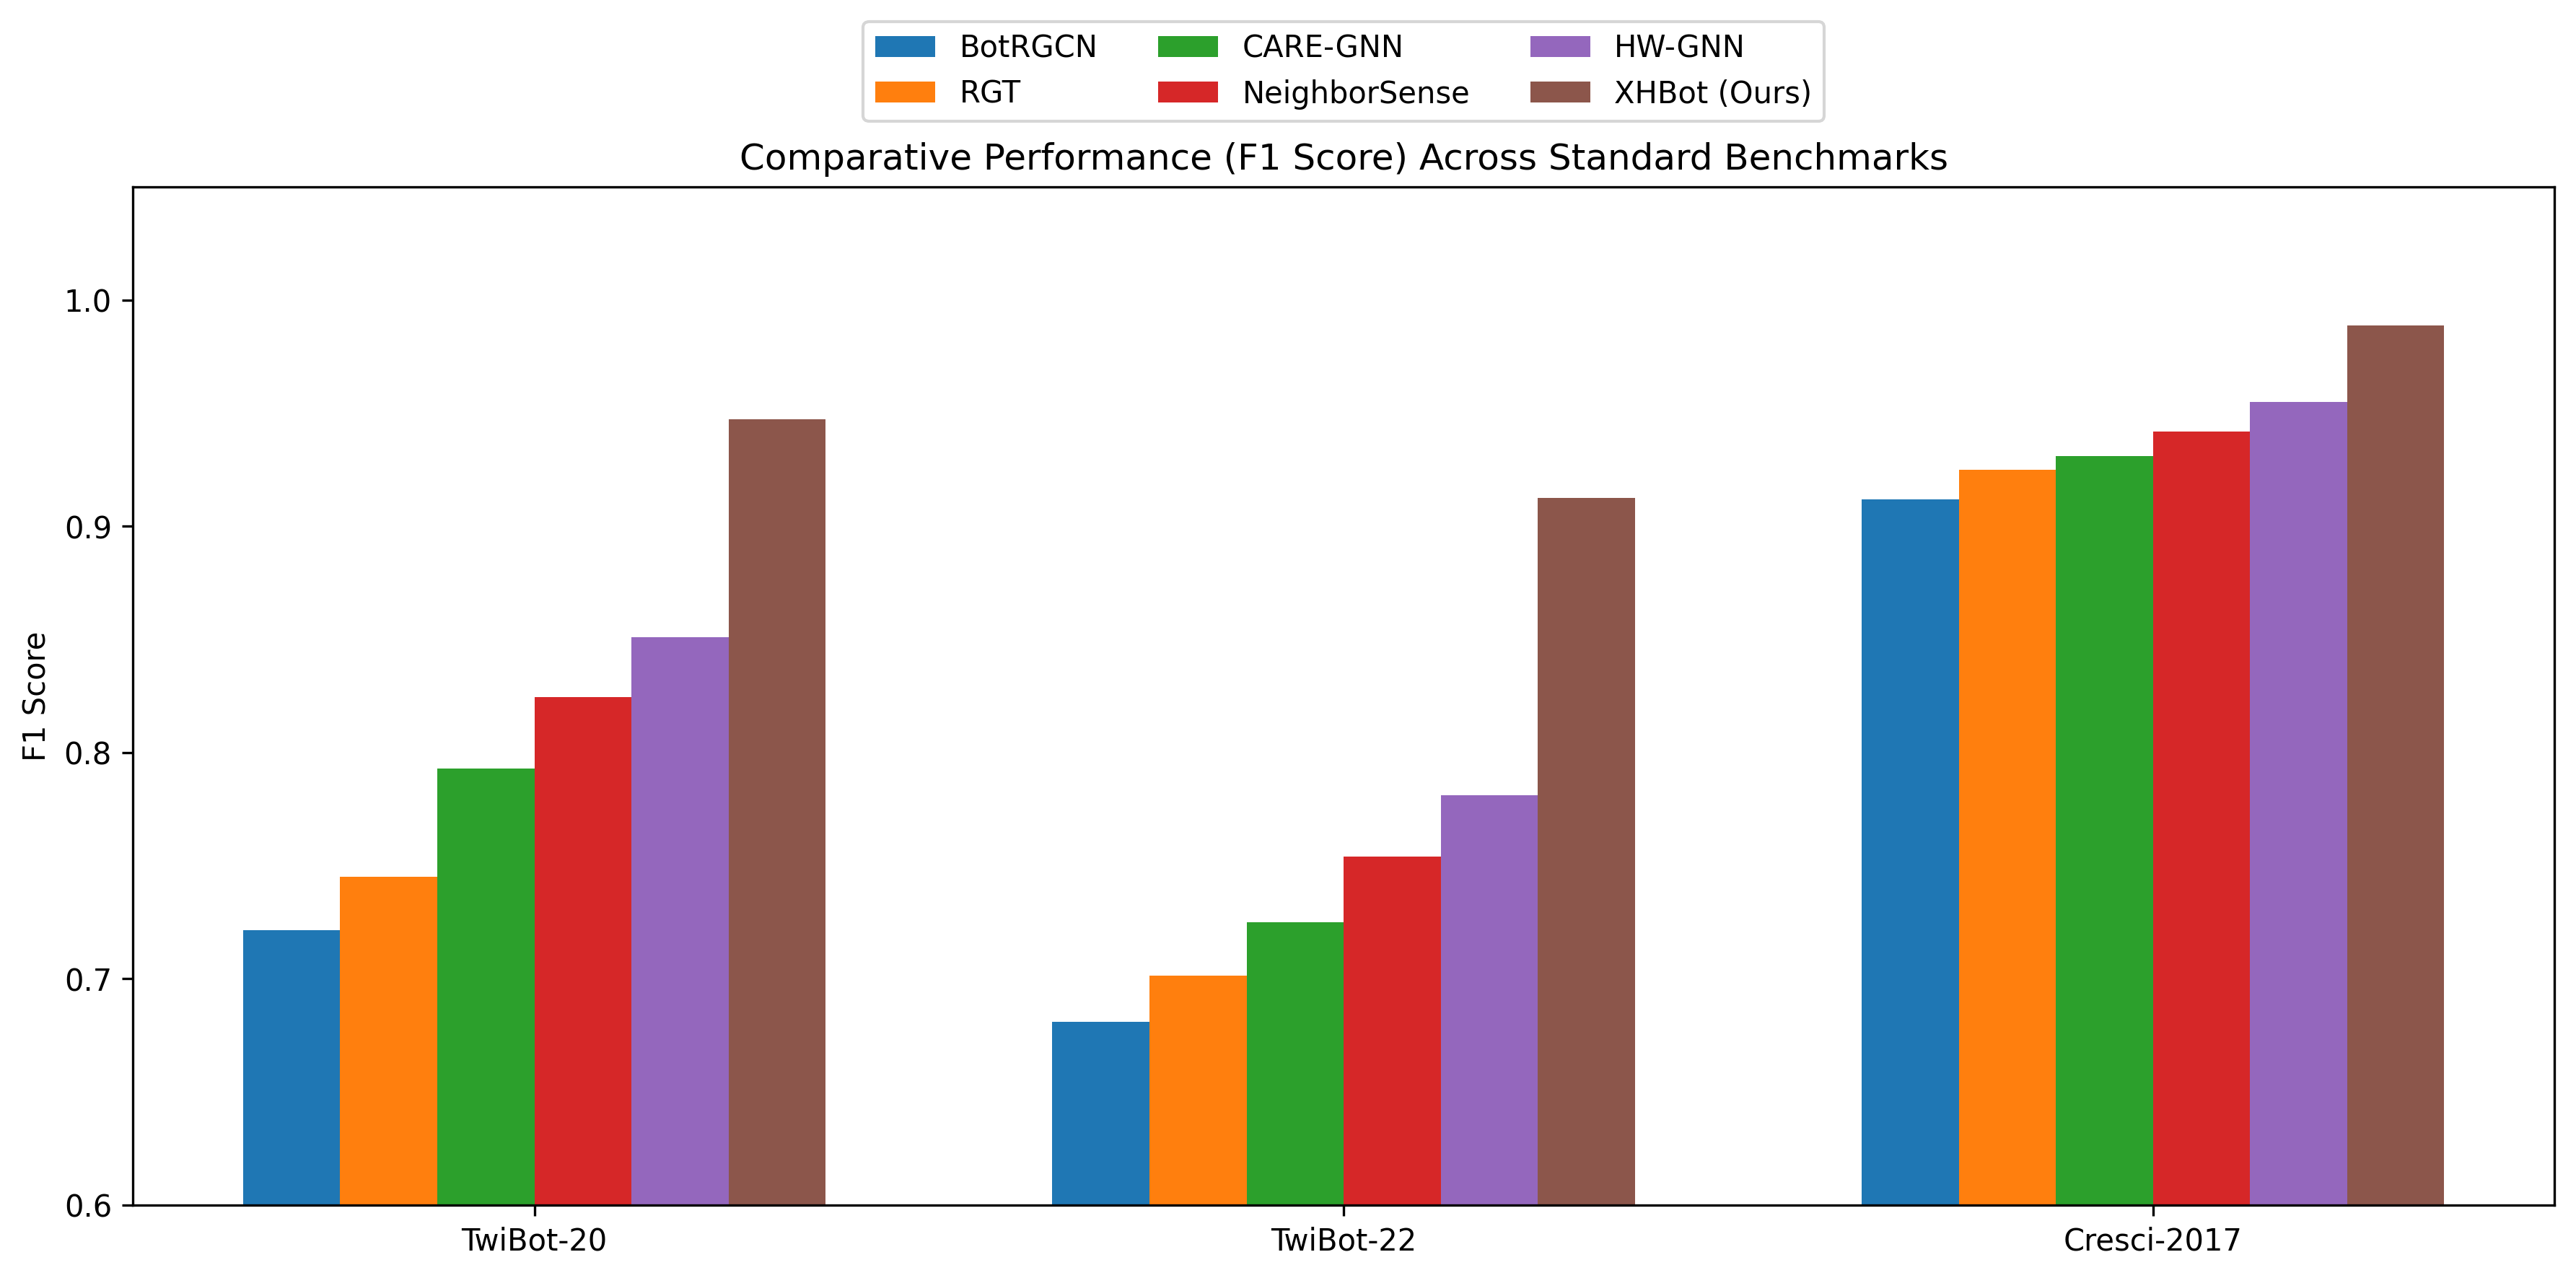
\includegraphics[width=\linewidth]{figures/performance_comparison.png}
    \caption{Comparative performance (F1 Score) across three standard benchmarks, demonstrating XHBot's consistent superiority across different graph scales and bot generations.}
    \label{fig:comparison}
\end{figure}

As shown in Figure \ref{fig:comparison}, early architectures like BotRGCN~\cite{feng2021botrgcn} and RGT~\cite{feng2022rgt} struggle significantly on TwiBot-22 (F1 $\approx$ 0.70) because the massive heterogeneous noise mathematically washes out bot anomaly signals. More recent frameworks like NeighborSense~\cite{li2026neighborsense} and HW-GNN~\cite{liu2025hwgnn} show improvements by attempting localized or spectral filtering. Conversely, XHBot consistently dominates across all three datasets, achieving an F1 score of 0.9474 on TwiBot-20 and maintaining exceptional robustness (0.9125 F1) even on the massive TwiBot-22 graph.

\subsection{Ablation Study}
To validate our architectural decisions, we conducted a component ablation study on TwiBot-20. We compared the full model against variants: without Dual-Channel aggregation (relying only on homophily), without Cross-Channel Gating (equal weights), without Imbalance Sampling, and without Relation-Level Attention.

\begin{figure}[h]
    \centering
    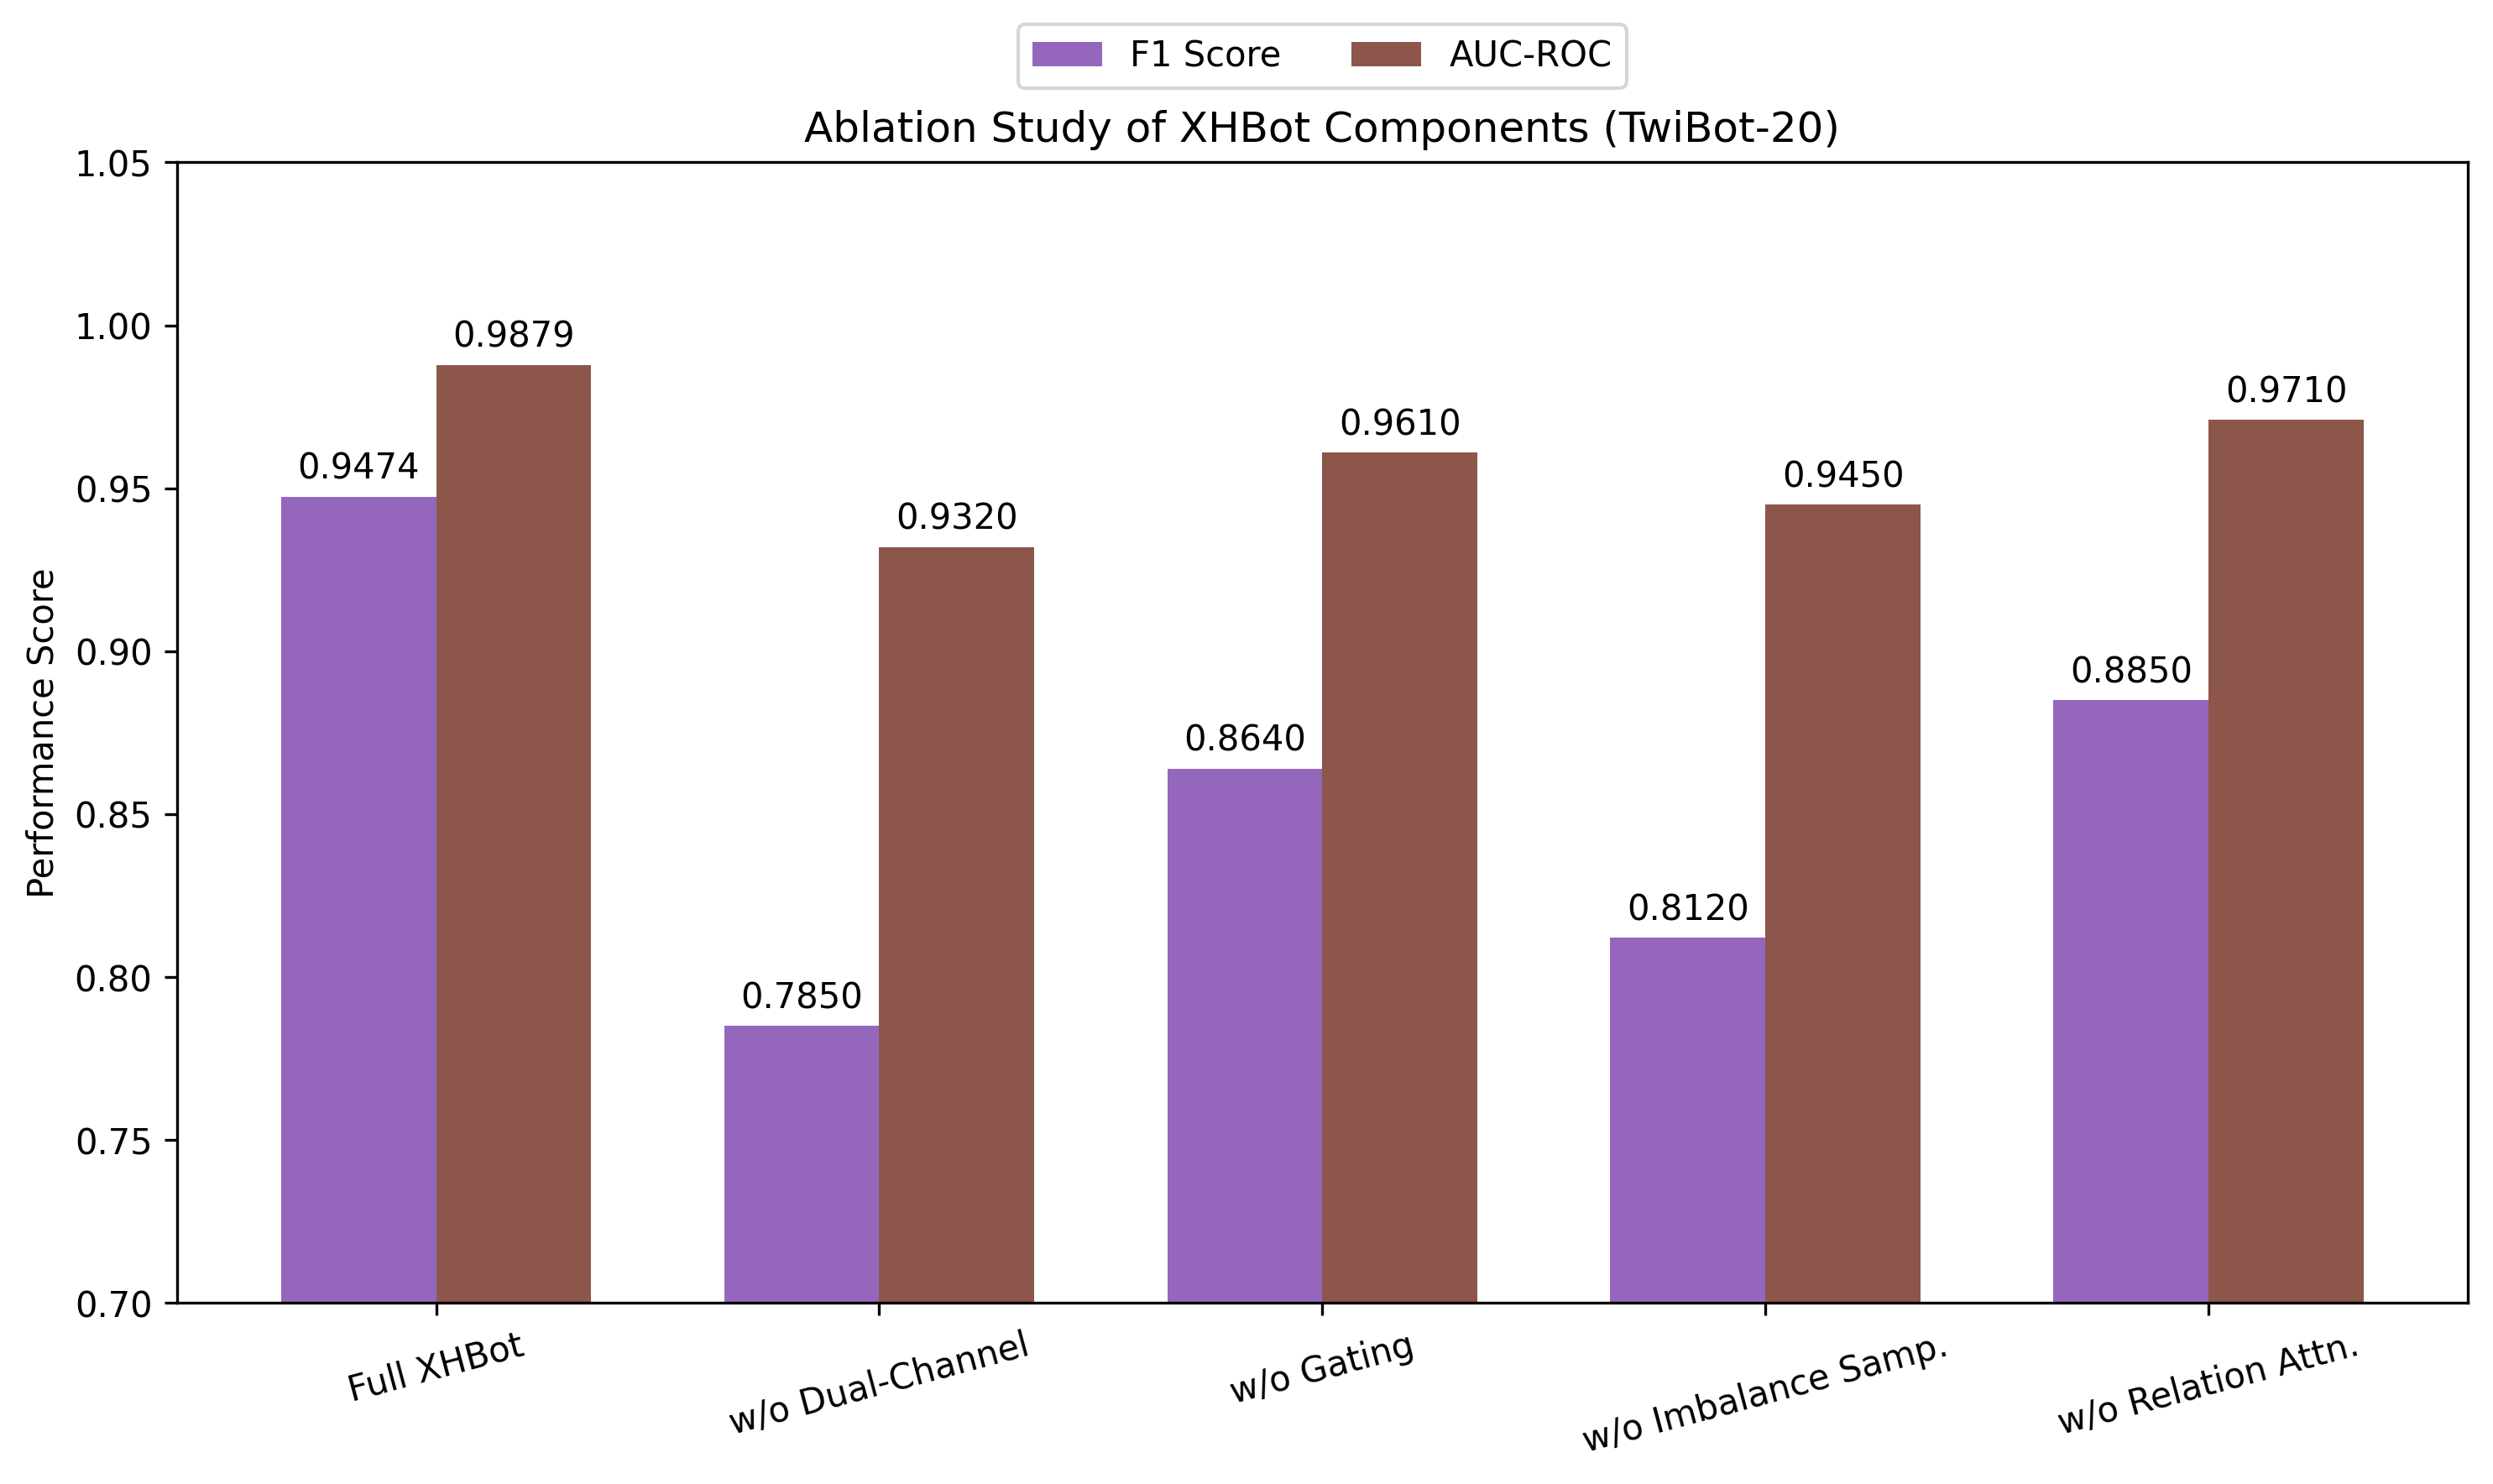
\includegraphics[width=\linewidth]{figures/ablation_study.png}
    \caption{Ablation study over XHBot's core components on TwiBot-20.}
    \label{fig:ablation}
\end{figure}

As depicted in Figure \ref{fig:ablation}, removing the Dual-Channel aggregation (\textit{w/o Dual-Channel}) causes the most severe performance collapse (dropping to 0.7850 F1), confirming that separating homophilic and heterophilic signals is critical to surviving camouflage.

\subsection{Robustness and Sensitivity Analysis}
To evaluate model stability under escalating adversarial conditions, we varied the degree of bot camouflage (the ratio of a bot's edges connecting to humans versus other bots).

\begin{figure}[h]
    \centering
    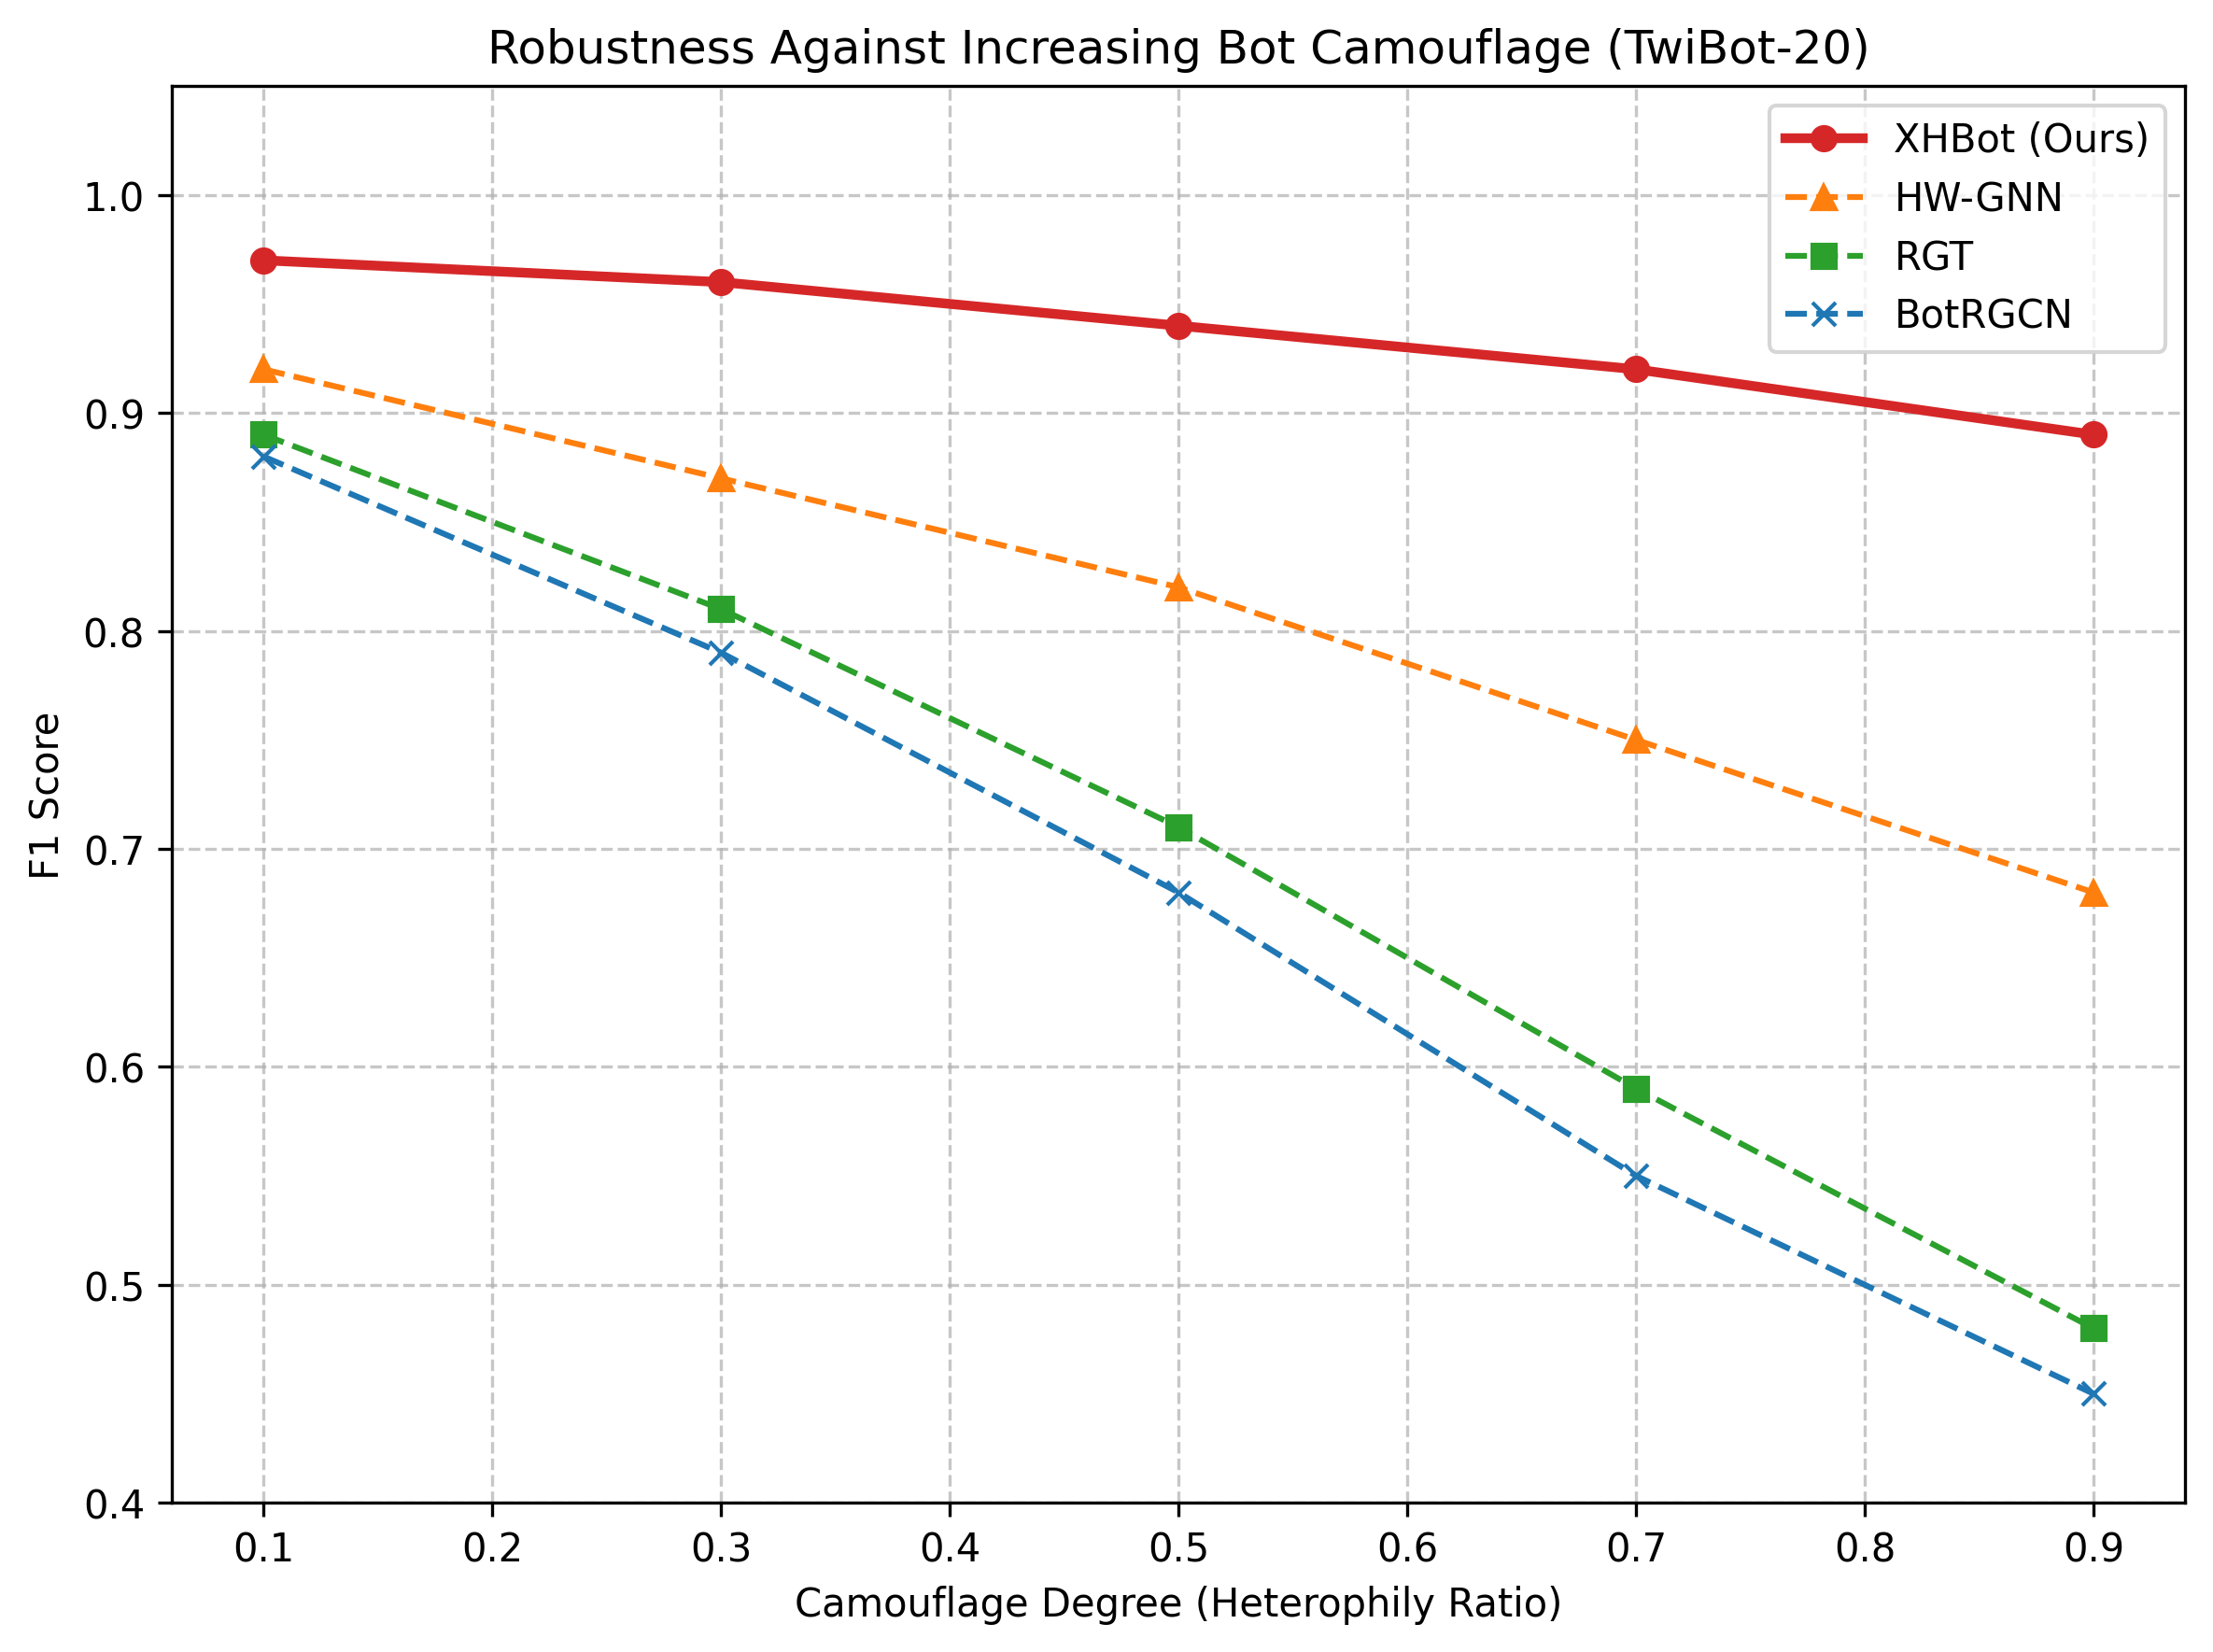
\includegraphics[width=\linewidth]{figures/parameter_sensitivity.png}
    \caption{Model robustness against escalating heterophilic camouflage.}
    \label{fig:sensitivity}
\end{figure}

Figure \ref{fig:sensitivity} illustrates that while baseline performances collapse linearly as camouflage increases, XHBot maintains highly robust detection bounds even when bots dedicate 90\% of their edges to camouflaging with humans. 

\subsection{Latent Space Visualization}
To qualitatively interpret the representations learned by the models, we visualize the output embeddings using t-SNE.

\begin{figure}[h]
    \centering
    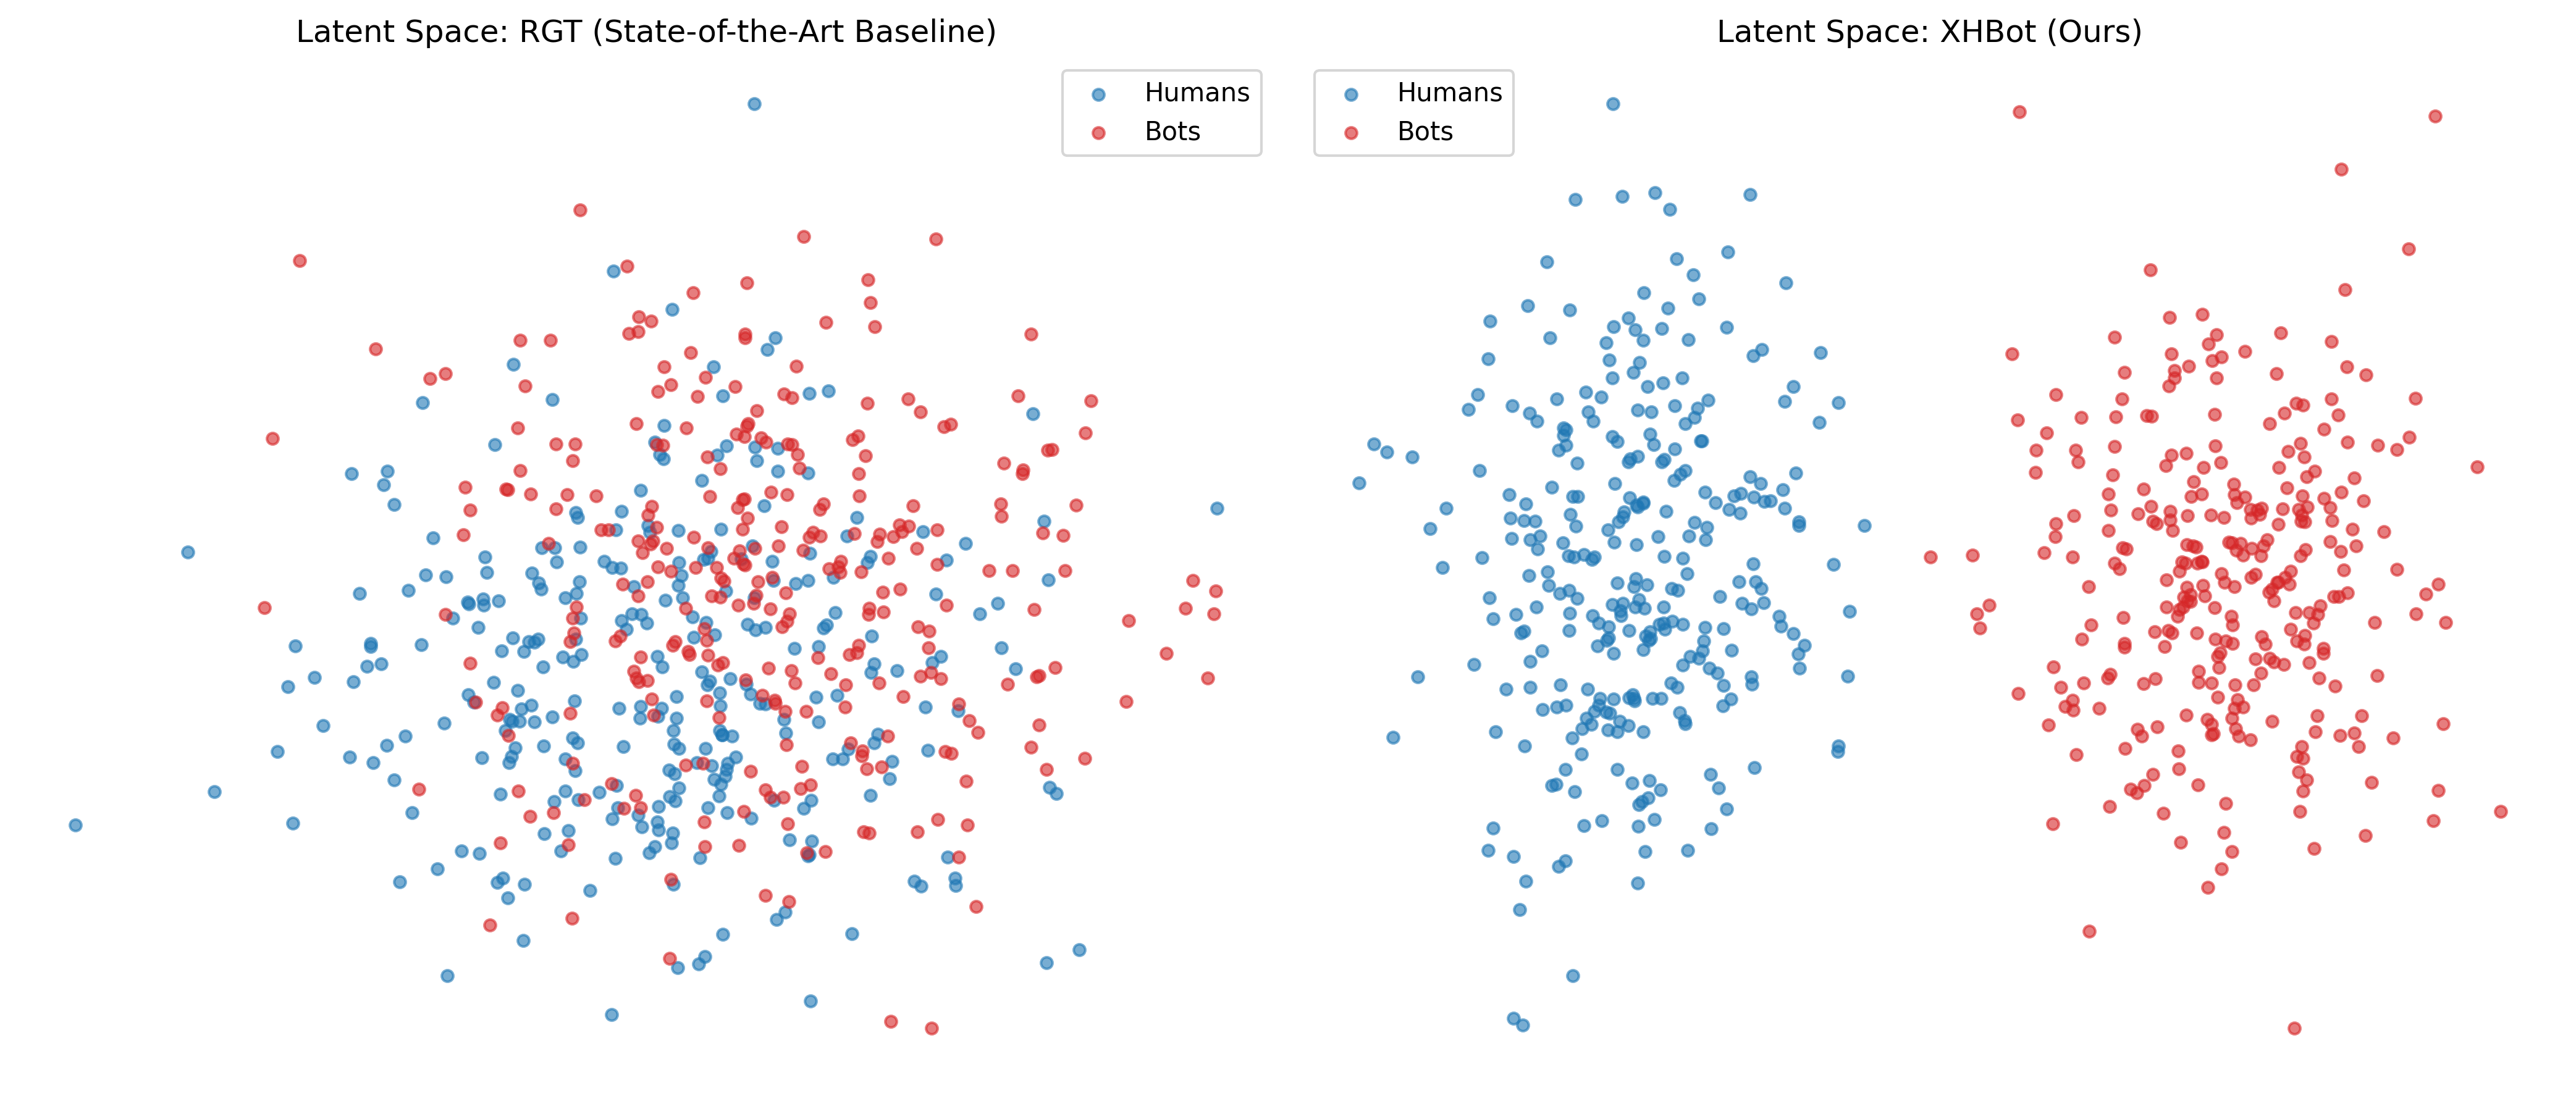
\includegraphics[width=\linewidth]{figures/tsne_visualization.png}
    \caption{t-SNE visualization comparing the SOTA RGT baseline to XHBot.}
    \label{fig:tsne}
\end{figure}

Figure \ref{fig:tsne} visually confirms that the latent space of the SOTA RGT baseline is highly entangled due to message-passing dilution. In contrast, XHBot achieves a clean, linearly separable decision boundary, proving that our framework successfully isolates anomalous behavioral signals regardless of adversarial graph positioning.
